\documentclass[14pt,reqno]{amsart}
\usepackage{extsizes}
%%%%%%%%%%%%%%%%%%%%%%%%%%%%%%%%%%%%%%%%%%%%%%%%%%%%%%%%%%%%%%%%%%%%%%%%%%%%%%%%%%%%%%%%%%%%%%%%%%%%%%%%%%%%%%%%%%%%%%%%%%%%%%%%%%%%%%%%%%%%%%%%%%%%%%%%%%%%%%%%%%%%%%%%%%%%%%%%%%%%%%%%%%%%%%%%%%%%%%%%%%%%%%%%%%%%%%%%%%%%%%%%%%%%%%%%%%%%%%%%%%%%%%%%%%
\usepackage{hyperref}
\usepackage{amsmath,amsfonts,amscd,amsthm,amssymb}
\usepackage{tikz,tikz-cd}
\usepackage{commath}
\usepackage[margin=1in]{geometry}
\usepackage{derivative}
\usepackage{enumitem}
\usepackage{changepage}
\usepackage{color,soul}
\usepackage{mathrsfs}
\setcounter{MaxMatrixCols}{10}
%\usepackage{pxfonts}
%\usepackage{txfonts}
\usepackage[T1]{fontenc}
\usepackage{mathptmx}
\usepackage{xeCJKfntef}
%\newtheorem{theorem}[subsection]{Theorem}
\newtheorem{thm}{Theorem}[section]
\newtheorem{prop}[thm]{Proposition}
\newtheorem{defi}[thm]{Definition}
\newtheorem{Remark}{Remark}[section]
\newtheorem{Example}{Example}[section]
\newtheorem{Lem}[thm]{Lemma}
\newtheorem{Coro}[thm]{Corollary}
\renewcommand{\proofname}{\text{Proof}}
\renewcommand{\figurename}{Fig.}
\numberwithin{equation}{section}
\usepackage{lipsum}  
\usepackage{graphicx}
\usepackage{float}
\begin{document}
	\begin{figure}
	\centering
	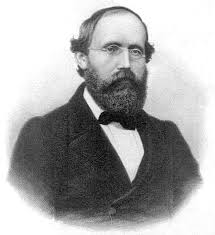
\includegraphics{Riemann.jpeg}
	\caption{Georg Friedrich Bernhard Riemann}
\end{figure} 
\begin{figure}
	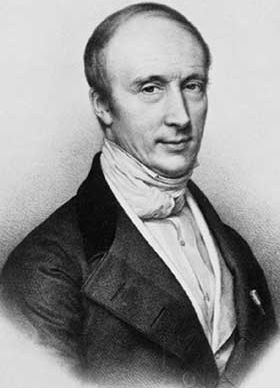
\includegraphics{Augustin-Louis_Cauchy_1901.jpg}
	\caption{Augustin Louis Cauchy}
柯西男爵抱有坚定的保皇信念和极端的宗教观点. 在他工作的这个活跃期间正值波旁王朝复辟,而在1830年的七月革命之后,柯西与皇族家庭一起移居到了意大利. 但到了1838年他返回了祖国并重新在一所天主教会学院里教数学,到了1848年他成了巴黎大学文理学院 (Sorbonne)的教授 (但他拒绝宣普效忠于政府)
\end{figure} 
\begin{figure}
	\centering
	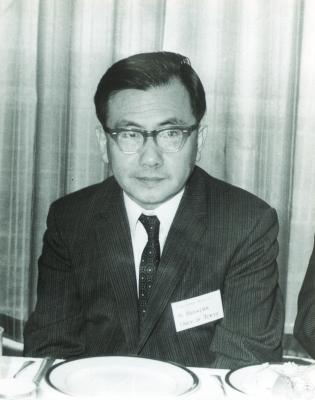
\includegraphics{Kodaira_Kunihiko.jpg}
	\caption{Kodaira Kunihiko(小平邦彦)}
\end{figure} 
\begin{figure}
	\centering
	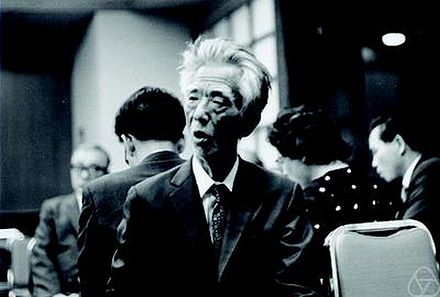
\includegraphics{440px-Kiyoshi_Oka.jpg}
	\caption{Kiyoshi Oka(冈洁)}
    1973年摄于京都
\end{figure} 

{\centering\section{Analytic Sets}}
		\begin{defi}\rm
			Let $G$ be a domain in $\mathbb{C}^{n}$, a close set  $A\subseteq G$ is called $\textbf{analytic set}$, if and only if for any $z\in A$, there exists an open set $V\subseteq G$ containing z and finite many holomorphic functions $\{f_{1},f_{2},,,f_{q}\}$,s.t. $Z(f_{1},f_{2},,,f_{q})=A\cap$V.
			\end{defi}
			\begin{prop}
				Let A be an analytic set in domain G, if A has a inner point,then $A=G$, else $G\backslash A$ is dense and connected.
				\begin{proof}
					(The proof is not complete, also considerting the case that A has countable infinite discrete points.)
					\\$\textbf{Case 1}$: Let G be a ball in $\mathbb{C}^{n}$ and $\{f_{1},,,, f_{q}\}$be a set of finite many holomorphic functions on defined on G s.t. $A=Z(f_{1},,,f_{q})$.
				\\If A has at least one inner point, then $\{f_{1},, f_{q}\}=\{0\}$, therefore $A=G$.
			\\If else, for any $z_{1},z_{2}\in G\backslash A$, let L be the unique complex line connecting $z_{1}$ and $z_{2}$, then $\{f_{1},, f_{q}\} |_{L}$ can be viewed as  a set of holomorphic funcitons of one variable, without loss of genelarity, assume that $L\nsubseteq Z(f_{1})$, then $L\cap Z(f_{1})$is discrete and therefore, ww can find a path in $L\subseteq G=B$ connecting $z_{1}$ and $z_{2}$, and avoiding A.(It a fact in algebraic topology.)
		\\$\textbf{Case 2}$: Let G be a general domain in $\mathbb{C}^{n}$,and assume that A has no inner point.\\
		For any path $\gamma$ in $G$ connecting $z_{1}$ and $z_{2}$, we can find finite open balls covering the path, then we can find an another path homotopic to $\gamma$ avoiding A.
		\end{proof} 
	\end{prop}
{\centering\section{Analytic Continuation}}	If A in analytic in domain G. we call A is proper iff $A\neq G$.
\begin{thm}	[\textbf{Riemann Continuation Theorem}]
	Let A analytic proper in domain $G\subseteq \mathbb{C}^{n}$, and f holomorphic in $A\nsubseteq G$, and f is locally bounded in any point $z\in A$, the f can be holomorphicly continuated to G.
	\begin{proof}
		Case 1: n=1. It's the known case in complex analysis of one variable.
		\\Case 2: n>1.For any $z_{0}\in A$we can find a complex $L$ through $z_{0}$,and $\textbf{locally}$ $L \cap A=\{z_{0}\}$.(why?).
		\\Through complex linear transformation and moving orign, $L$ satisfies the system$\{z_{2}=z_{2}=...=z_{n}=0\}$
		Let $r_{1}$,$r^{'}$ be suffiently small positive numbers s.t.
		\begin{equation*}
			\begin{aligned}
				P=\{z=(z_{1},z^{'})\in\mathbb{C}\times\mathbb{C}^{n-1}|z^{'}=(z_{2},,,z_{n}), |z_{1}|<r_{1}, |z^{'}|<r^{'}\} \subseteq G.
			\end{aligned}
		\end{equation*}
		and $A\cap\{z\in \mathbb{C}^{n}|\ |z_{1}|=r_{1}, |z^{'}|<r^{'}\}=\emptyset$,
		moreover for any $0\leq c\le r_{1}$, $A\cap\{z\in \mathbb{C}^{n}|\ |z_{1}|=r_{1}, |z^{'}|<c\}$can be viewed as the intersection $\mathbb{D}\cap A$. Then through the one dimensional case, we can continuate f on  $G\backslash A$  holomorphicly to $P$ and therefore to $G$. 
	\end{proof}
\end{thm}
{\centering\section{Regular Points of Analytic Sets}}
\begin{defi}\rm
	Let G be a domain in $G\subseteq \mathbb{C}^{n}$, A is locally defined at $z_{0}\in A$ by $Z(f_{1},f_{2},,,f_{q})$where $f_{i}\in \mathcal{O}(G)$, then $rank_{z_{0}}(f_{1},f_{2},,,f_{q}):=rank(J(f_{1},f_{2},,,f_{q})(z_{0}))=rank(\dfrac{\partial f_{i}}{\partial z_{j}}(z_{0}))\leq q$.
	If such $\{f_{1},f_{2},,,f_{q}\}$ exists and $rank_{z_{0}}(f_{1},f_{2},,,f_{q}=0)$ we call A is regular q codimensional at $z_{0}$. $z_{0}$is called a regular point of A. All regular points called the regular set of A(written as $A_{reg}$), the set of other points is called singluar set.($A_{sing}$) 
\end{defi}
\begin{thm}	[\textbf{local parameterization}]
	Let A analytic in domain$G\subseteq \mathbb{C}^{n},z_{0}\in A$, then A is q codimensional regular at \textbf{iff} at $z_{0}$ G is locally biholomorphic to an open set $W\subseteq\mathbb{C}^{n}$ centered at the orign, and the biholomorphic map satisfies:
	$F(z_{0})=0$and $F(U\cap A)=\{w=(w_{1},,,w_{n})|\ w_{n-q+1}=...=w_{n}=0\}$
	\begin{proof}
		The proof is similiar to the proof of implict function theory and omitted here.
 	\end{proof}
\end{thm}
It is obvious that $A_{reg}$ is open in A.
\begin{thm}
	Let G be a domain of $\mathbb{C}^{n}$,and $f\in \mathcal{O}(G)$and $f$is not constant, then $Z(f)$ has at least one regular point.
	\begin{proof}
		Case 1: n=1, obvious.\\
		Case 2: n>1.  Assume that $A=Z(F)=\emptyset$,then $df=0$ on $A$.
	\\For any $z_{0}\in A$, we can always find $n_{0}\in \mathbb{N}_{+},$ and a multiplied index $v_{0}$, and $\lambda\in\{1,2,,,n\}$,s.t $|v_{0}|=n_{0}$ and $(D^{v_{0}}f)(z_{0})\neq0$,moreover $D^{v}f)(z)=0$ for any $z\in A$, $|v|\leq n$
	we define $M=\{z\in G|\ D^{v_{0}}f(z)=0\}$, then $A\subseteq M$ and M is regular at $z_{0}$.
	Through a local parameterization  at $z_{0}$, we have $z_{0}=0$ and $M=\{z=(z_{1},,,z_{n})|\  z_{1}=0\}$, then $f(\zeta,\vec{0})\neq0$ for $|\zeta|\neq0$and small enough. Using \textbf{Argument principle}, we notice that viewing $z_{0}$ as variable, for $|\vec{\zeta}|<r$ small enough. $f(\eta,\vec{\zeta})$has zero points in ball $|\vec{\zeta}|<r$,and therefore  the points fall in A. Consequently, we have $A=M$. This leads to the contradiction.
 	\end{proof}
\end{thm}
\end{document}